\section{Music libraries and listening habits} % (fold)
\label{sec:listening_behaviour}

% The previous chapter has made clear that Internet holds a deep knowledge of the way in which people experience music and that this knowledge can be automatically retrieved and analysed to better understand the associations that subsist between songs and artists.

Different persons are characterised by different listening behaviours: some are used to play all kinds of music in a shuffled order, others to listen only to a particular genre; some are eager to discover the latest trends of contemporary music, others are obsessed with playing the same album again and again.

The previous chapter focused on music organised in playlists.
Some persons do not use playlists at all but decide in real time which songs to play in their music devices.
The simple fact of a person picking a particular song to play is already a musical experience that is worth be analysed.

The wide proliferation of digital music players has made it easy to track the history of a listener.
Most digital players (Apple iTunes, iPod, Winamp, Windows Media Player, etc.) store data about each played song; Apple iTunes, for instance, records the play count (number of times the song was played), the play recency (last time the song was played), the skip count (number of times the song was skipped before its end) and the user rating for each song in the music library (see Fig.~\ref{fig:itunes_claudio}).
%
\begin{figure}[bthp]
\centering \setlength{\abovecaptionskip}{3pt}
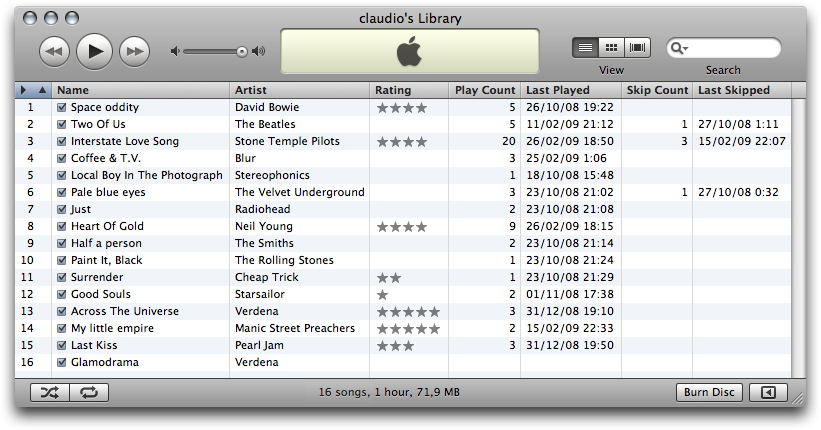
\epsfig{file=img/itunes_claudio, width=\textwidth}
\caption{Personal music library managed with iTunes.}
\label{fig:itunes_claudio}
\end{figure}

Listening behaviour data is very descriptive of personal preferences: 
having played certain songs and not other ones outlines the musical taste of an individual better than a verbal description, with its inaccuracies and misinterpretations, would.

As many persons share their listening behaviour data on the Internet to make their friends aware of their musical habits, the Web has become the best place where to find data about which songs a person has played, when, how they were rated, et cetera.
%For example, the list of songs I have been listening to in the last four years is publicly available in my Last.fm profile page. % LINK

%This chapter presents a technique that, given listening behaviour data of any individual, is able to identify that person's favourite songs and, generically, to \emph{measure how much} that individual shows to like each available song.

The purpose of this chapter is to introduce a measure of \textbf{musical preference} that automatically estimates how much a person likes a given song based on personal listening habits data collected from the Web.

% Sharing this data on the Internet is simple, thanks to tools that automatically connect personal music libraries to the Web, tracking and publishing in real time data about the music played.
% %
% To know which music a person likes is then a matter of finding that person's listening history on the Web and analysing the retrieved data to identify which songs that person prefers.
% 
% The purpose of this chapter is to present a technique to transform listening habits data into a degree of musical preference that measures \emph{how much} each individual shows to like each song.
% 
%The advantage of this technique is that it models musical preferences just observing how music has been \emph{experienced} rather than asking for a verbal description of musical taste.

% Many persons make their listening behaviour data public by sharing them in online communities. This is done through automatic tools that detect songs in personal digital players and publish their usage data on the Web.
% MusicStrands, for instance, provides a software called MyStrands that works both with Apple iTunes and Windows Media Player.
% Similarly, Last.fm provides a tool called Audioscrobbler that tracks all the songs reproduced in digital and portable players (Apple iTunes, Windows Media Player, Winamp, iPod, iPhone, Android) to show them on Last.fm member pages.
% 
% Tracking individual listening behaviour data is very helpful to understand which kind of music a person likes.
% The actual \emph{experience} of selecting a particular set of songs to play from a possibly large music library offers a valuable hint about which music a person likes.
% In my opinion, \emph{observing} what a person plays is more valuable than \emph{asking} about one's musical taste, since verbal descriptions are more subject to inaccuracy and misinterpretation. 
% 
% The goal of this chapter is the following: given a group of people $\mathcal{U}$ and a set of songs $\mathcal{C}$ obtain from the Web experience data about how each member $U \in \mathcal{U}$ has been listening to each song $X \in \mathcal{C}$ and, from this data, measure \emph{how much} each person likes each song in the set.
% 
% The purpose is to show how the musical preferences of each individual can be modelled just with data that describes how a person \emph{used} music in the past, without the need to verbally state which music a person likes best.


 
% Listening behaviour data intrinsically reveals a valuable personal experience.
% The goal of this chapter is to explain how this experience can be analysed in order to estimate the preferences of an individual for a set of songs and artists.
% 
% The purpose of this chapter is to introduce a technique to measure the \textbf{musical preferences} of an individual based on the analysis of listening behaviour data included in personal music library.
% 
% The approach that I propose consists in (1) retrieving personal music libraries from the Internet, and (2) analysing the intrinsic listening behaviour to determine which songs and artists each listener mostly prefers.
% 
% Sect.NN reviews previous works on user modelling, comparing two strategies to build a profile of individual preferences. Sect.NN ..

% section listening_behaviour (end)

\section{Previous work} % (fold)
\label{sec:user_modelling_techniques}

The issue faced in this chapter consists in identifying a set of individual musical preferences without having to explicitly ask for them.
The process of acquiring user preferences is known as user modelling \cite{Rich79,Kass88,Kobsa01} and can either be explicit or implicit.

\subsection{Explicit user modelling} % (fold)
\label{sub:explicit_models}

Explicit acquisition of preferences is obtained when individuals \emph{actively} provide specific facts about loved items.
Most online stores, for instance, ask their users to provide feedback about purchased items: Amazon collects ratings about books, Trip Advisor about travel destinations, eBay about sellers' reputation.

Explicit feedback is the most direct way for users to express their taste, although \citet{Claypool01} noticed how having to stop to enter explicit ratings can alter normal patterns of information usage, and \citet{Zhang02} proved how users can rapidly stop providing explicit ratings unless they perceive a benefit. 
Amazon and eBay, for instance, gratify frequent raters highlighting their profiles as `experts' within the community of users.

 \citet{Potter08} also pointed out how explicit statements require users to `translate' their inner preferences into a score, which is not an immediate and unequivocal process: deciding how many `stars' to assign to a good item is a matter of personal interpretation.
\citet{Banerjee92} also noticed that users asked to rate an item are easily influenced by the scorings assigned by previous users. % \emph{Herding}  refers to the fact that and, as shown in \cite{Cosley03}, this can worsen future recommendations about that item.

% subsection explicit_models (end)

\subsection{Implicit user modelling} % (fold)
\label{sub:implicit_models}

Implicit user modelling % is the alternative approach to explicit preferences described in this chapter and 
takes place by \emph{observing} user actions and inferring preferences from the observed behaviours.
For instance, someone always buying clothes in the same store implicitly expresses a preference for that fashion style. 
Similarly, forwarding an online video to ten friends implicitly demonstrates an interest for that video. %, regardless of any assigned rating.

In different publications, \citet{Nichols97}, \citet{Oard01} and \citet{Kelly03} have categorised several types of actions as possible sources for implicit user modelling.
Figure~\ref{fig:implicit-feedbacks} reports the list of actions according to the underlying purpose of the observed action (Behaviour Category), and to the smallest possible scope of the item being acted upon (Minimum Scope).
In the domain of music, for instance, having either purchased, saved, rated or listened a specific song can be interpreted as an implicit preference for that song.

\begin{figure}[bthp]
\centering \setlength{\abovecaptionskip}{3pt}
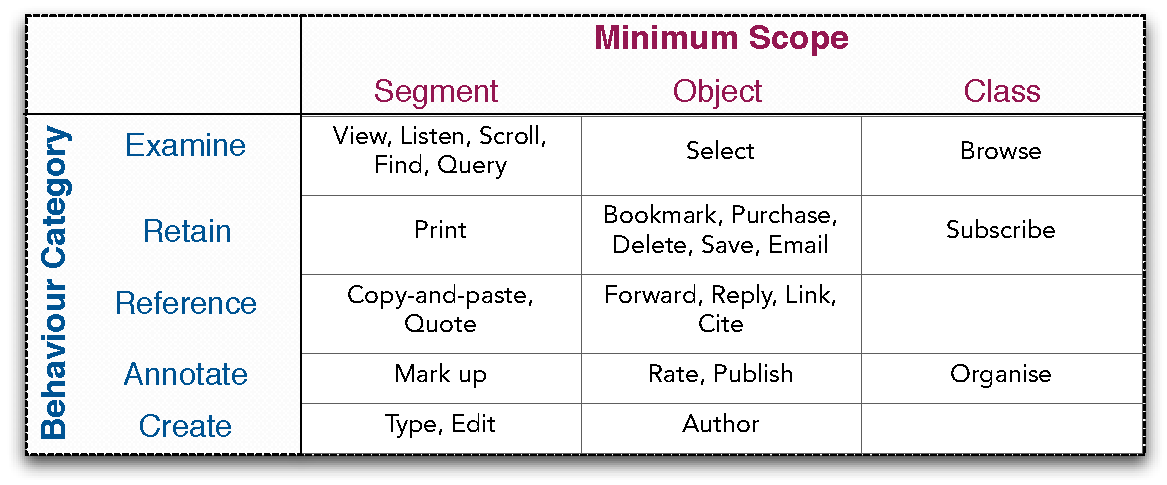
\epsfig{file=img/fig3_2, width=\textwidth}
\caption{Classification of behaviours used to infer implicit feedback.}
\label{fig:implicit-feedbacks}
\end{figure}

% subsection implicit_models (end)

\subsection{Building user profiles} % (fold)
\label{sub:building_user_profiles}

Collecting implicit or explicit preferences is only the first step to compile a comprehensive model of user preferences.
As pointed out by \citet{Hofmann04}, different users associate different meanings with ratings; for instance, `4 out of 5 stars' may have a different meaning for different people. 
For this reason, individual preferences need be \emph{normalised} in order to be compared. 
%\cite{Hu07b} demonstrated how almost all products in Amazon have an asymmetric bimodal (J-shaped) distribution with more positive than negative reviews.
\citet{Goldberg01} proposed to normalise each rating by subtracting its mean rating over all users, and then dividing by its standard deviation.

Another relevant aspect of user modelling is how to build a comprehensive model when only a few individual preferences are available.
\citet{Dieterich93} suggested to either start with an \emph{empty} model, to classify the user into one \emph{stereotypical} category, or to build an initial \emph{individual} model based on a preliminary question-answering session. 
A stereotypical approach, for instance, is used by Last.fm which uses geographical position obtained from the IP address of unregistered users to  recommend musical events taking place in the area where users are located.

Interests may change along time, so a system that learns a model of the user's interests should be based on algorithms that can quickly adjust to changing interests.
The notion of changing target concepts is known as ``concept drift'' \cite{Billsus07}, or ``persistence of interest'' \cite{Lieberman95}.
\citet{Dieterich93} distinguished between ``short-term'' data\,---\,user preferences that are valid only for the current context or session\,---\,and ``long-term'' data\,---\,which should be kept beyond the current session and saved in a permanent storage medium. 
In the domain of music, for instance, Last.fm online radio differentiates between `skipping' a song (short-term negative preference) and `banning' a song (long-term negative preference) from a personalised music channel.

% [Talk about explicit approaches for preferences, like photo Identikit]

% subsection building_user_profiles (end)

% section user_modelling_techniques (end)

%% section problem_description2 (end)
% 
% \section{Explicit approach} % (fold)
% \label{sec:explicit_approach}
% 
% The easiest way to determine how much a person would like to listen to a specific song in a radio channel is through direct feedback.
% Poolcasting Web Radio offers a Web interface that allows anyone to express a personal evaluation about the songs available on a channel (Fig.~\ref{fig:pwr_rate}).
% By clicking on the `Good' and `Bad' buttons , listeners can express their explicit preferences.
% %
% \begin{figure}[bthp]
% \centering \setlength{\abovecaptionskip}{3pt}
% \epsfig{file=img/radio_rate, width=\textwidth}
% \caption{Poolcasting Web Radio allows explicit song rating.}
% \label{fig:pwr_rate}
% \end{figure}
% 
% The \textbf{explicit preference} is denoted as the function $e: \mathcal{U} \times \mathcal{C} \times \mathbb{N}^+ \to [-1,1]$, where a positive (resp., negative) value $e(U,X,T)$ indicates that a participant $U$ would (resp., would not) like a song $X$ to be played on the channel at time $T$, and a value of zero denotes indifference.
% 
% Initially, the explicit preference is null for each listener $U \in \mathcal{U}$ and each song $X \in \mathcal{C}$.
% As participants express their explicit feedback, poolcasting updates these values accordingly.
% To express a slightly positive preference for a song $X$, a participant $U$ clicks \emph{once} the `Good' button, and the explicit preference is updated to $e(U,X,T) = 0.5$. Clicking \emph{twice} or more the `Good' button is interpreted as a strong positive preference, and stored as $e(U,X,T) = 1$.
% Similarly, clicking once on the `Bad' button results in $e(U,X,T) = -0.5$, while clicking twice or more results in $e(U,X,T) = 1$.
% Clicking first on `Good' and then on `Bad' or vice versa resets the value to $e(U,X,T) = 0$.
% 
% %In this way, listeners can express either a very negative, negative, null, positive, or very positive preference for any song by means of two feedback buttons.
% 
% The reason why the explicit preference $e(U,X,T)$ is a function of time $T$ is because participants can change their mind about a song over time; for instance a participant might initially love to hear `Holiday' by Madonna played on a channel and, after a certain time, might not care about `Holiday' being played since another song by Madonna has been broadcast meanwhile.
% 
% The time $T \in \mathbb{N}^+$ represents the number of songs played on the channel so far; when a channel is created $T = 0$, when the first song has been played $T = 1$, and so on. 
% The explicit preference $e(U,X,T)$ corresponds to the most recent statement expressed by the listener $U$ about the song $X$ at time $T$.
% 
% \begin{example}
% A participant $U$ listens to a radio channel broadcasting music from the Eighties.
% After three songs, $U$ wishes song $X$ `Holiday' by Madonna to be played, so $U$ clicks once on `Good', resulting in $e(U,X,3) = 0.5$.
% After two more songs, $U$ wishes song $Y$ `True Colors' by Cyndi Lauper to be played, so $U$ clicks twice on `Good', resulting in $e(U,Y,5) = 1$.
% After three more songs, $U$ becomes indifferent about `Holiday' being played, since another song by Madonna has been broadcast meanwhile, so $U$ clicks once on `Bad', updating the explicit preference to $e(U,X,8) = 0$.
% \end{example}
% 
% Explicit statements are the most direct way for poolcasting to gather individual musical preferences.
% Nevertheless, most radio listeners do not wish to spend a lot of time and effort in evaluating the songs proposed by the radio.
% For this reason, poolcasting integrates this explicit approach with an implicit approach that can estimate the musical taste of each participant without requiring any interaction.
% % section explicit_approach (end)
% 
\section{Gathering listening habits} % (fold)
\label{sec:implicit_approach}

To determine individual music preferences from the analysis of personal listening habits, these have to be collected first, which can occur in two ways.

The first method is to extract this information directly from personal music libraries. 
Apple iTunes, for instance, stores in the hard disk a file called `iTunes Library.xml' which describes the list of played songs, play counts, play recency, skip counts, user ratings.
Parsing this XML file provides first-hand knowledge about the music played on that particular machine.

The second method is to gather this knowledge from the Internet.
Different tools track personal listening habits and make these data available on the Web.
Last.fm, for instance, provides each member with a Web page showing the last songs played, the device where they were played and the assigned rating, as detected by the music tracking software Audioscrobbler (see Fig.~\ref{fig:lastfmprofile}).
MusicStrands offers a similar service with a tool called MyStrands (see Fig.~\ref{fig:musicstrands}).
%
\begin{figure}[bthp]
\centering \setlength{\abovecaptionskip}{3pt}
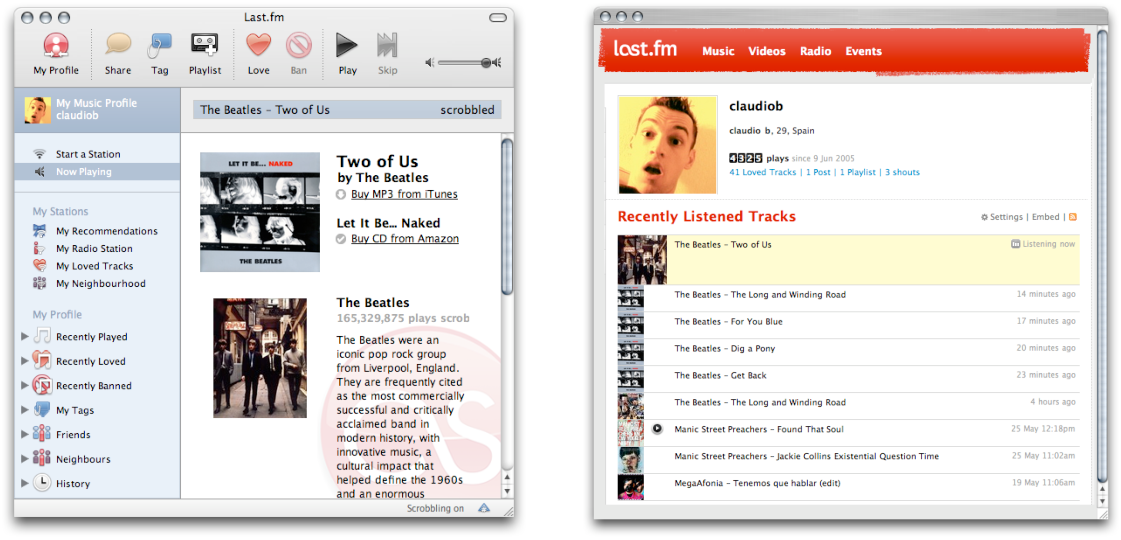
\epsfig{file=img/lastfm, width=\textwidth}
\caption{Last.fm tracking tool Audioscrobbler and profile Web page.}
\label{fig:lastfmprofile}
\end{figure}
%
\begin{figure}[bthp]
\centering \setlength{\abovecaptionskip}{3pt}
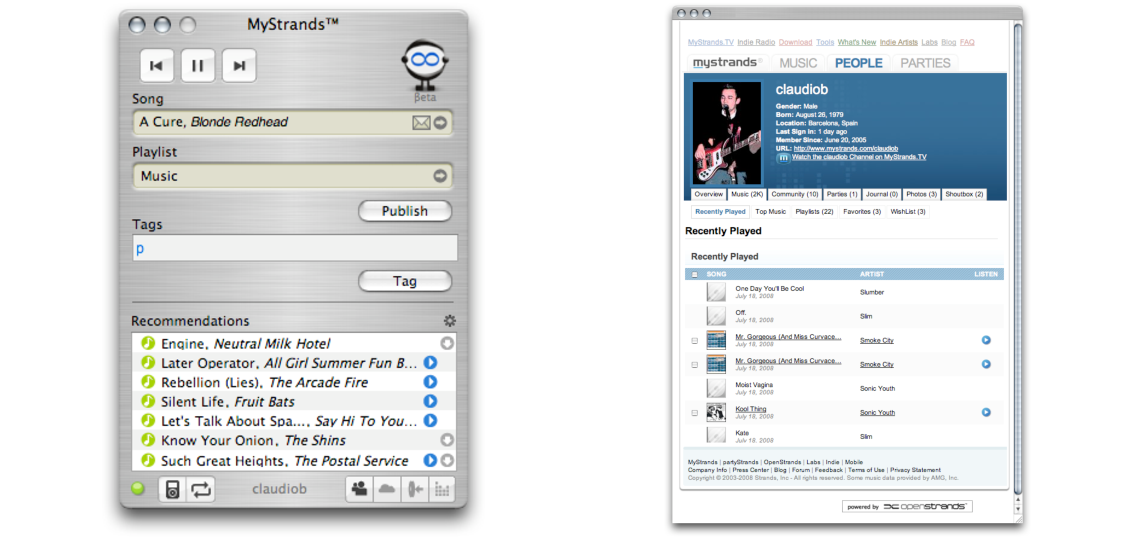
\epsfig{file=img/musicstrands, width=\textwidth}
\caption{MusicStrands tracking tool MyStrands and profile Web page.}
\label{fig:musicstrands}
\end{figure}

Gathering listening habits from the Web has four main advantages.
Firstly, data can be collected from thousands of users without having to access their hard disks.
Secondly, Web services provide Web Application Programming Interfaces (API) \cite{Booth04} to rapidly retrieve large amount of data in a standard XML format.
Thirdly, Web services can automatically fix mistakes in song titles (e.g., `Obladi Oblada' rather than `Ob-la-di Ob-la-da') thus correctly identifying played songs.
Fourthly, Web services can automatically aggregate the listening habits from multiple devices; for instance Last.fm `scrobbles' both songs played in portable devices (iPod, iPhone, Android) and digital libraries (iTunes, Windows Media Player, Winamp).


%The next section will explain how the play count and rating of each song can effectively be combined to estimate the degree in which a person likes that song.

% There are several Web communities that allow people to share their listening behaviours online, and most of them provide tools to rapidly gather this knowledge for different users.
% Last.fm, for instance, provides a Web API [CITE] that gives direct access to the list of songs played by any member of Last.fm in a tracked device.
% Similarly, MusicStrands offers the OpenStrands API to access individual listening behaviour data.
% 
% The granularity of information stored by these communities is not uniform. Last.fm, for instance, reports when each member played each song, on which device, and whether the song was rated or skipped; OpenStrands reports only about played songs and ratings.
% 
% Of all the listening behaviour data that can be collected online about a person, there are two properties that most clearly identify which music a person most likes: \textbf{user ratings} and \textbf{play counts}. 
% The simple fact that a song has been (1) rated positively and (2) played many times denote an interest of the listener for that song.
% Other properties are more subject to noise; for example the fact of \emph{skipping} a playing song is not necessarily related to the preference for that song, that song might just not fit well in the current musical context.
% 
% In brief, the Web contains a lot of experience data about which songs were played by different persons. Given a person $U \in mathcal{U}$ and a song $X \in \mathcal{C}$, information can be extracted regarding how $U$ rated song $X$ and how many times $U$ listened to $X$. 
% This information can be used to estimate the degree in which $U$ shows to prefer song $X$, as will be presented in the following section.
% 

\section{Estimating individual preferences} % (fold)
\label{sec:estimating_individual_preferences}

Once listening habits data have been collected, a choice has to be made about which part of these data can be considered as illustrative of music preferences.

One relevant property is clearly the \textbf{user rating} assigned to each song. 
Almost every digital player enables listener to vote for favourite songs; Apple iTunes uses `stars' (from 1 to 5), while Audioscrobbler gives the option to mark a song as either `Loved' or `Banned'.

A second relevant property is the \textbf{play count}: how many times a song was played. Intuitively, the interest of a person for a song is directly related to its play count, especially if the song has been played often recently.

Other relevant properties, such as the skip count and the play recency, will not be utilised since they are more subject to interpretation. % than user rating and play count. 
Skipping a song, for instance, might be interpreted as a negative preference, but listeners also skip songs they like when these do not fit in the current context. 

The rest of this section explains how, given the ratings assigned by a person to a set of  songs and their play counts, a measure of \textbf{individual preference} for each song can be defined.

\subsection{Usage behaviour normalisation} % (fold)
\label{sub:usage_behaviour_normalisation}

Let $\mathcal{U}$ be a group of people and let $U \in \mathcal{U}$ be a person for which listening habits data are available with respect to a set of songs  $\mathcal{C}$.
Let $r: \mathcal{U} \times \mathcal{C} \to [\varrho_{\min}, \varrho_{\max}]$ be the rating assigned by $U$ to each song, where $\varrho_{\min}$ and $\varrho_{\max}$ are the minimum and maximum rating scores (e.g., $\varrho_{\min} = 1$ and $\varrho_{\max} = 5$ `stars' in Apple iTunes), and
let $n: \mathcal{U} \times \mathcal{C} \to \mathbb{N}$ be the play count, that is, the number of times that $U$ played each song.

The goal is to combine for each song $X \in \mathcal{C}$ the two values $r(U,X)$ and $n(U,X)$ in order to measure the \textbf{individual preference} degree $i: \mathcal{U} \times \mathcal{C} \to [0,1]$, that is, how much $U$ shows to like song $X$.

High ratings and high play counts identify songs a listener likes. 
The `absolute' values of rating and play count, though, offer small information to estimate a preference degree.
%
Having listened to a song 3 times or having assigned a rating of `3 out of 5' stars, for instance, do not clearly indicate whether a listener likes a song or not. If that listener normally rates songs with only 1 or 2 stars, then giving 3 stars expresses a positive preference. 
If the average rating is instead 4 or 5 stars, then 3 stars is probably not a good signal.
Similarly, a play count of 3 is significant or not whether the listener is a sporadic or a frequent music listener.

User ratings and play counts are values that are relevant only with respect to the \emph{average listening behaviour}.
Only songs showing a play count or a rating above the average can significantly be considered as favourite songs.
For this reason, user ratings $r(U,X)$ and play counts $n(U,X)$ are hereafter \emph{normalised} to yield values in the range $[-1,1]$, so that only songs `above the average' are assigned positive values.


\subsection{Normalising user rating} % (fold)
\label{sub:normalising_user_rating}


To define a \emph{normalised user rating} means to find a function  $\widehat{r}: \mathcal{U} \times \mathcal{C} \to [-1,1]$ which returns positive (resp., negative, null) values for songs rated higher than (resp., lower than, equal to) the average. 
Let $\mathcal{R}_U \subseteq \mathcal{C}$ be the songs that a person $U \in \mathcal{U}$ has ever rated and let
%
\begin{equation*}
   \overline{r(U)} = \frac{\sum_{X \in \mathcal{R}_U} r(U,X)}{\#(\mathcal{R}_U)}       
\end{equation*}
be the average user rating of $U$.
The normalised user rating $\widehat{r}(U,X)$ is a function that satisfies these conditions:
\begin{equation}\label{eq:normalisation_conditions_1}
\left\{ \begin{array}{lll}
\rule[-1em]{0pt}{2.5em}
r(U,X) < \overline{r(U)} & \implies & -1 < \widehat{r}(U,X) < 0 \\
\rule[-1em]{0pt}{2.5em}  
r(U,X) = \overline{r(U)} & \implies & \widehat{r}(U,X) = 0 \\
\rule[-1em]{0pt}{2.5em}  
\overline{r(U)} < r(U,X) & \implies & 0 < \widehat{r}(U,X) < 1
\end{array} \right.
\end{equation}
and such that any song with the lowest (resp., highest) possible rating obtains the minimum (resp., maximum) possible normalised value:
\begin{equation}\label{eq:normalisation_conditions_2}
\left\{ \begin{array}{lll}
\rule[-1em]{0pt}{2.5em}
r(U,X) = \varrho_{\min}  & \implies & \widehat{r}(U,X) = -1 \\ 
%\rule[-1em]{0pt}{2.5em}  
%r(U,X) = \overline{r(U)} & \implies & \widehat{r}(U,X) = 0 \\
\rule[-1em]{0pt}{2.5em}  
r(U,X) = \varrho_{\max} & \implies & \widehat{r}(U,X) = 1%\,,
\end{array} \right.
\end{equation}
under the condition that $\varrho_{\min} < \overline{r(U)} < \varrho_{\max}$.

% Formally, I indicate with $i: \mathcal{U} \times \mathcal{C} \to [0,1]$ the \textbf{implicit preference} inferred by poolcasting from usage behaviour [ ONLY FROM $o$, right?], where $i(U,X)$ refers to how much a participant $U$ shows to like an item $X$: the higher the value, the more $U$ shows to like $X$. %, a value of 0 denotes indifference.
% 
% Formally, let 
% then $U$ implicitly likes every song $X \in \mathcal{L}_U$ used more than the average:
% \begin{equation}\label{eq:infer_implicit}
% \left\{ \begin{array}{lll}
% 	\rule[-1em]{0pt}{2.5em}  
% 	r(U,X) \leqslant \overline{r(U)} & \implies & i(U,X) = 0\\
% 	\rule[-1em]{0pt}{2.5em}  
% 	r(U,X) > \overline{r(U)} & \implies & i(U,X) > 0\,.\\
% \end{array} \right.
% \end{equation}
% 
% 
% Let $\widehat{r}: \mathcal{U} \times \mathcal{C} \to [-1,1]$ be the normalised version of the observed usage property $o$.
% Items showing a usage property higher than (respectively, lower than) the average are assigned a positive (resp., negative) normalised value:
% 
% Items showing exactly an average usage property are assigned a normalised value of $0$; other items are assigned a normalised value of $-1$ (respectively, $1$) only if they show the lowest (resp., highest) possible usage property values:
% where:

One function that fulfils \eqref{eq:normalisation_conditions_1} and \eqref{eq:normalisation_conditions_2} and is furthermore continuous, monotonic, derivable, with the first derivative monotonic in the interval $(-1,1)$ is the function that solves the following linear equation system:
\begin{equation*}%\label{eq:linear_system}
\left\{ \begin{array}{ll}
\rule[-1em]{0pt}{2.5em}
a\log(b + \varrho_{\min}) + c = -1\\
\rule[-1em]{0pt}{2.5em}
a\log(b + \overline{r(U)}) + c = 0\\
\rule[-1em]{0pt}{2.5em}
a\log(b + \varrho_{\max}) + c = 1
\end{array} \right.
\end{equation*}
and that yields $0$ when $r(U,X) = \overline{r(U)}$.
The solution of this system is defined by cases:
\begin{equation*}
\widehat{r}(U,X) = 
\begin{cases}
%\rule[-1em]{0pt}{2em} 
%-1 
%& \text{if $\overline{r(U)} = \varrho_{\min}$}\\        
\rule[-1em]{0pt}{2em} 
0 
&\hspace{-2em}\text{if $r(U,X) = \overline{r(U)}$}\\   
\rule[-1em]{0pt}{3em} 
\cfrac{2(r(U,X) - {\varrho_{\med}}^2)}{\varrho_{\max} -\varrho_{\min}} 
&\hspace{-1em}\text{if $\overline{r(U)} = \varrho_{\med}$}\\
\rule[-1em]{0pt}{6em} 
\cfrac{\log\cfrac{2r(U,X)(\varrho_{\med} - \overline{r(U)}) + \overline{r(U)}^2 - \varrho_{\max}\varrho_{\min}}{(\varrho_{\max} - \overline{r(U)})(\overline{r(U)} - \varrho_{\min})}}
 {\log(\varrho_{\max} - \overline{r(U)}) - \log(\overline{r(U)} -  \varrho_{\min})} 
& \text{otherwise,}
\end{cases}
\end{equation*}
where $\varrho_{\med} = \frac{1}{2}(\varrho_{\min} + \varrho_{\max})$. % (e.g., 3 stars in iTunes). % is the median possible value for the property.
%


The three cases defining $\widehat{r}(U,X)$ are separately illustrated in Fig.~\ref{fig:normalisation_function} and depend on the average rating $\overline{r(U)}$ of each person $U$:
\begin{itemize}
 \item when $U$ assigns the same rating to every song, then 
$r(U,X) = \overline{r(U)}$ for every song and $\widehat{r}(U,X)$ falls back to the constant $0$ (solid line in Fig.~\ref{fig:normalisation_function});
% \item when $U$ has the maximum usage behaviour possible for every item, then $\overline{r(U)} = \varrho_{\max}$ and $\widehat{r}(U,X)$ falls back to the constant $1$ (higher dotted line in Fig.~\ref{fig:normalisation_function});
 \item when $U$ has an average rating of $\varrho_{\med}$, then $\widehat{r}(U,X)$ falls back to a linear function (dashed line in Fig.~\ref{fig:normalisation_function}); % with zero-cross in $X = \varrho_{\med}$; 
 \item otherwise $\widehat{r}(U,X)$ is a logarithmic function, concave or convex whether the average rating $\overline{r(U)}$ is higher or lower than $\varrho_{\med}$ (dotted lines in Fig.~\ref{fig:normalisation_function}). 
\end{itemize}
%
\begin{figure}[bthp]
\centering \setlength{\abovecaptionskip}{3pt}
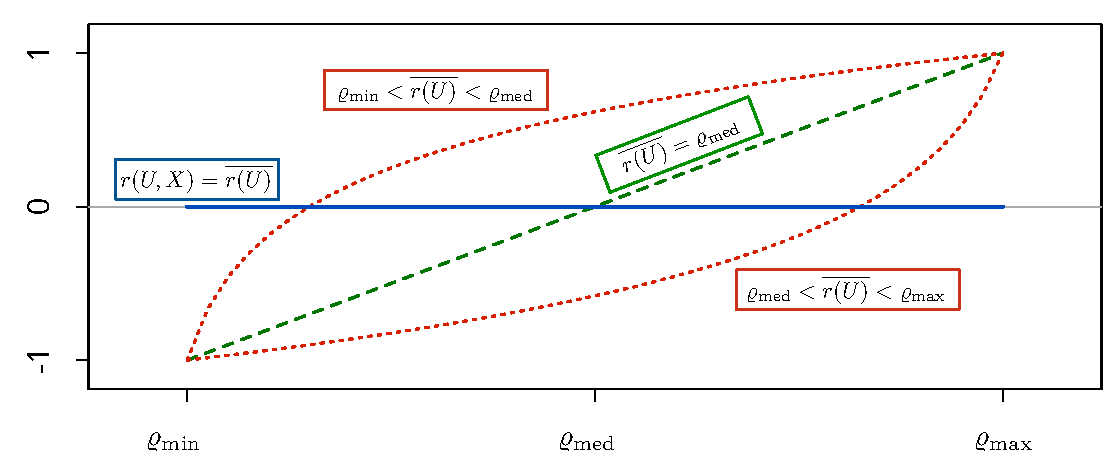
\epsfig{file=img/fig3_5, width=\textwidth}
\caption{Normalised user ratings corresponding to different values of $\overline{r(U)}$.}
\label{fig:normalisation_function}
\end{figure}
Working with normalised values, every rating is interpreted with respect to each user, and the same absolute rating (e.g., 4 stars) can assume different normalised values $\widehat{r}(U,X)$ for different people.

\begin{example}
Figure~\ref{fig:compared_normalisation} represents the situation where two friends $U$ and $V$ have both listened to ten songs $\mathcal{C} = \{X1, X2, \ldots, X10\}$ and have rated them with different criteria.
Even though $U$ and $V$ both assigned four stars to song $X5$, the normalised user rating for this song differs: $\widehat{r}(U,X5) = 0.67$ is positive, while $\widehat{r}(V,X5) = 0$ is not.
The reason is that $U$ assigns in average two stars to each song, so the observed value $r(U,X5) = 4$, higher than the average, corresponds to a positive normalised user rating, while $V$ assigns in average four stars to every song, so the observed value $r(V,X5) = 4$ is not equally significant.
%
\begin{figure}[bthp]
\centering \setlength{\abovecaptionskip}{3pt}
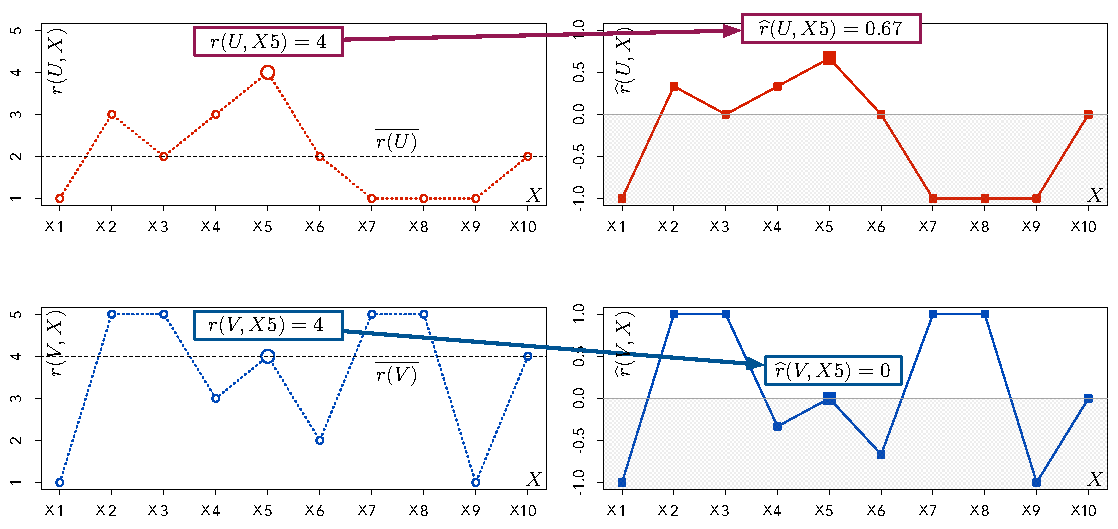
\epsfig{file=img/fig3_6, width=\textwidth}
\caption{Effect of the normalisation process on user ratings.}
%xample of two participants $X$ and $Y$ showing equal behaviour $o$ for the same item $X5$ but having different normalised values $\widehat{r}$.} 
\label{fig:compared_normalisation}
\end{figure}
        
\end{example}

% subsection usage_behaviour_normalisation (end)

\subsection{Combining user ratings and play counts} % (fold)
\label{sub:positive_and_negative_implicit_preferences}

Following the same approach described to normalise user ratings, play counts $n(U,X)$ can be normalised as well, resulting in a normalised play count function $\widehat{n}: \mathcal{U} \times \mathcal{C} \to [-1,1]$ that yields positive (resp., negative, null) values for songs played more than (resp., less than, as much as) the average play count.

Normalising user ratings and play counts helps identify songs for which a person has a particular interest: 
every song $X$ for which $\widehat{r}(U,X) > 0$ or $\widehat{n}(U,X) > 0$ has obtained by $U$ a rating or play count higher than the average and, as such, can be assessed as one of the songs preferred by $U$.

Formally, the \textbf{individual preference} degree $i: \mathcal{U} \times \mathcal{C} \to [0,1]$ that measures how much $U$ likes each song $X \in \mathcal{C}$ is defined as a linear combination of these normalised properties:
\begin{equation}\label{eq:implicit_preference}
i(U,X) = \pi \cdot \max(0,\widehat{r}(U,X)) + (1 - \pi) \cdot \max(0,\widehat{n}(U,X)) % \max(0,\widehat{o_J}(U,X))
\end{equation}
where $\pi \in [0,1]$ denotes the importance assigned to ratings with respect to play counts.

The reason why both normalised rating and play count are limited to a minimum value of zero is that implicit preferences are assessed only for songs for which either the rating or the play count is above the average.
No `negative' assumption is made about songs rated or played less than average.
The reason is that a person may have not rated or played a specific song for several reasons (lack of time, of a digital player, of the right occasion) and this should not be always interpreted as a lack of interest.
On the other hand, having taken the effort to rate or play often a song should be positively interpreted as an implicit measure of interest.

This technique allows to estimate individual music preferences without any explicit action by the listener, exploiting only knowledge implicit in the listening habits data of a person.

\begin{example}
The music library shown in Fig.~\ref{fig:itunes_claudio} contains 8 rated songs, with an average rating of 3.5 stars; five songs were rated above this value.
Similarly, 15 songs have been played, the average play count is 4 and four songs have a play count above this value.
The implicit preference of the author for these songs can be calculated with the function \eqref{eq:implicit_preference} assigning the same importance to ratings and play counts ($\pi = 0.5$).
The results are reported in Table~\ref{table:itunes}:
`Interstate Love Song' (Stone Temple Pilots) stands out as the author's favourite song, followed by `Across The Universe' (Verdena) and `My Little Empire' (Manic Street Preachers). 
A song such as `Last Kiss' (Pearl Jam) is not in the list because both its rating (3 stars) and its play count (3) fall below the average.
\end{example}

%\vspace{0.3cm}
\begin{table}[bhtp]
\centering \setlength{\abovecaptionskip}{3pt}
\caption{Individual preferences assessed for songs in Fig.~\ref{fig:itunes_claudio}.}\label{table:itunes}
\begin{tabular}{|cc|c|c|c|c|c|}
\hline
\multicolumn{2}{|c|}{song}&\multicolumn{2}{c|}{rating}&\multicolumn{2}{c|}{play count}&preference\\
\multicolumn{2}{|c|}{$X$}&$r(U,X)$&$\widehat{r}(U,X)$&$n(U,X)$&$\widehat{n}(U,X)$&$i(U,X)$\\
\hline

\multirow{2}{*}{3}  & \small{Interstate} & \multirow{2}{*}{4} & 
\multirow{2}{*}{0.28} & \multirow{2}{*}{20} & \multirow{2}{*}{1} & \multirow{2}{*}{\textbf{0.64}}\\ & \small{Love Song} &&&&& \\ \hline

\multirow{2}{*}{13}  & \small{Across The} & \multirow{2}{*}{5} & 
\multirow{2}{*}{1} & \multirow{2}{*}{3} & \multirow{2}{*}{0} & 
\multirow{2}{*}{\textbf{0.50}}\\ & \small{Universe} &&&&& \\ \hline

\multirow{2}{*}{14}  & \small{My Little} & \multirow{2}{*}{5} & 
\multirow{2}{*}{1} & \multirow{2}{*}{2} & \multirow{2}{*}{0} &
\multirow{2}{*}{\textbf{0.50}}\\ & \small{Empire} &&&&& \\ \hline

\multirow{2}{*}{8}  & \small{Heart} & \multirow{2}{*}{4} & 
\multirow{2}{*}{0.28} & \multirow{2}{*}{9} & \multirow{2}{*}{0.5} & 
\multirow{2}{*}{\textbf{0.39}}\\ & \small{Of Gold} &&&&& \\ \hline

\multirow{2}{*}{1}  & \small{Space} & \multirow{2}{*}{4} & \multirow{2}{*}{0.28} & \multirow{2}{*}{5} & \multirow{2}{*}{0.12} & \multirow{2}{*}{\textbf{0.20}}\\ & \small{Oddity} &&&&& \\ \hline

\multirow{2}{*}{2}  & \small{Two} & \multirow{2}{*}{---} & 
\multirow{2}{*}{---} & \multirow{2}{*}{5} & \multirow{2}{*}{0.12} & \multirow{2}{*}{\textbf{0.12}}\\ & \small{Of Us} &&&&& \\ \hline


\end{tabular}
\end{table}
%\vspace{0.3cm}



% 
% The normalised function $\widehat{r}(U,X)$ represents how a person $U$ rated a song $X$ with respect to the average individual rating.
% If $U$ has assigned to $X$ a rating higher than the average, then $\widehat{r}(U,X)$ is positive, and a positive implicit preference can be assessed for $X$.
% If $U$ has assigned to $X$ a rating lower than the average, then no assumption should be done about implicit preferences.
% Therefore the implicit preference of a user $U$ for a song $X \in \mathcal{L}_U$ can be estimated from the user rating $r(U,X)$ as the function:
% \begin{equation}\label{eq:implicit_one}
% 	\max(0, \widehat{r}(U,X))\,.
% \end{equation}
% which returns positive values for songs rated more than the average, and returns 0 for songs rated equal or less than the average.
% 
% % According to \eqref{eq:infer_implicit}, poolcasting infers a positive implicit preference in this case. 
% % %Poolcasting uses this value to quantify the implicit preference for each item $X \in \mathcal{L}_U$.
% % Given one observable property $r(U,X)$, poolcasting estimates the implicit preference of participant $U$ for an item $X$ as:
% % \begin{equation*}
% % \begin{cases}
% % \rule[-1em]{0pt}{2em} 
% % i(U,X) = \widehat{r}(U,X) & \text{if $\widehat{r}(U,X) > 0$}\\        
% % \rule[-1em]{0pt}{2em} 
% % i(U,X) = 0 & \text{otherwise.}
% % \end{cases}
% % \end{equation*}
% % This formula can be written in a more compact style as:
% 
% % subsection positive_and_negative_implicit_preferences (end)
% 
% \subsection{Inferring implicit preference from multiple usage properties} % (fold)
% \label{sub:combining_multiple_observable_properties}
% 
% Star rating is just one of the way people express their listening behaviours.
% As shown in Fig.~\ref{fig:itunes_claudio}, digital libraries store more usage behaviour data than just user ratings.
% By combining many of these properties, a more comprehensive degree of implicit preference can be obtained.
% For instance, an implicit preference can be assessed for any song rated more than 3 stars, listened at least twice and skipped no more than 4 times.
% 
% 
% %Participants might show more than one observable usage behaviour property at the same time; for instance poolcasting might know \emph{both} the number of times a person listened to a song \emph{and} how many friends that song was recommended to. In this case, poolcasting infers implicit preference through a linear combination of normalised behaviour values.
% 
% Let $N$ be the number of observable properties of a participant $U$ for an item $X \in \mathcal{L}_U$ (e.g., user rating, play count), let $o_1, o_2, \ldots, o_N$ be their absolute values, and let $\widehat{o_1}, \widehat{o_2}, \ldots, \widehat{o_N}$ be their respective normalised values.
% The function $i: \mathcal{U} \times \mathcal{C} \to [0,1]$ that estimates the \textbf{implicit preference} of a participant $U$ for a song $X$ based on all the observed properties is defined as:
% \begin{equation}\label{eq:implicit_preference}
% i(U,X) = \sum_{J=1}^N \pi_J \cdot \max(0,\widehat{o_J}(U,X)) % \max(0,\widehat{o_J}(U,X))
% \end{equation}
% where the parameters $\pi_J \in [0,1]$ denote the importance assigned to each observable property, under the constraint that $\sum_{J=1}^N \pi_J = 1$.

% subsection combining_multiple_observable_properties (end)


% \section{The application} % (fold)
% \label{sec:the_application}
% 
% [Here explain a minimum of iTunes format and an example with my own library, with my average usage etc.] 
% More evaluation and tuning of parameters available in Chap7.
% 
% For instance if I combine rating and play count in the iTunes library before I get these values..
% 
% % section the_application (end)

% ction{Explicit statements} % (fold)
% bel{sec:explicit_statements}
% 
% ITHER THIS GOES HERE OR AT THE BEGINNING ]
% 
%  method presented so far allows to infer preferences without asking the individuals. However these preferences are only positive, while a user might want so explicitly state that a song is not appreciated.
% o, these preferences are static, calculated only once, while a user might want to update and change them.
% o these preferences are generic, not specific to a channel. In particular, if iTunes library is analysed, then implicit preferences only about songs you like at work, at home, etc., can be assessed.
% 
% 
%  all these reasons, explicit statements are also permitted...
% 
% 
% ection explicit_statements (end)
%


% subsection contributions5 (end)

\subsection{Integrating additional properties} % (fold)
\label{sub:expanding_to_artists3}

The individual preference degree \eqref{eq:implicit_preference} combines only two observable properties: user ratings and play counts.
Other observable properties can be easily integrated in the function if they are found to be significantly related to musical preferences.
%
The skip count (number of times a song was skipped before its end), for instance, can be considered as an indicator of `negative' preferences.
This property can be included into \eqref{eq:implicit_preference} by first normalising its values to the range $[-1,1]$, then adding this value to the linear combination \eqref{eq:implicit_preference} that defines the value of $i(U,X)$.
The only precaution is to invert negative preferences: songs skipped \emph{less} than the average would yield a positive normalised value and vice versa.

\subsection{Extending to artists} % (fold)
\label{sub:expanding_to_artists2}

Whatever the number of properties considered, songs that have never been `experienced' (played, rated, skipped) are always assigned a value of $i(U,X) = 0$, which means that no implicit preference can be assessed.

This is an intrinsic limitation of the proposed technique: preferences can only be inferred for songs in the individual listening history.
This behaviour can be improved considering that, in general terms, a person has similar preferences for songs by the same artist.
For instance, if $U$ has assigned 5 stars to ten songs by Bj\"{o}rk, then $U$ will probably like future released by Bj\"{o}rk as well, since $U$ shows to enjoy her music. 
In other words, a positive implicit preference for $U$ can be assessed for \emph{any} song by Bj\"{o}rk, even those that $U$ has not yet heard.

Formally, let $X$ be a song that a person $U$ has not yet experienced, and let $\mathcal{Y}_U(X)$ be other songs by the same artist of $X$ that $U$ has experienced:
\begin{equation}
   \mathcal{Y}_U(X) = \{Y\,|\,a(X) = a(Y)\,\wedge\,i(U,X) = 0\}\,.
\end{equation}
Then, the individual preference of $U$ for song $X$ can be estimated as the average preference for known songs by the same artist:
%
\begin{equation*}
        i(U,X) = \sum_{Y \in \mathcal{Y}_U(X)} \frac{i(U,Y)}{\#(\mathcal{Y}_U(X))}\,.
\end{equation*}
%
This extension enables the definition of a degree of implicit preferences also for songs outside of a personal music library.

% subsection expanding_to_artists2 (end)

\section{Summary} % (fold)
\label{sec:contributions5}

This chapter has presented a technique to build individual music profiles from the analysis of personal listening habits.
%
Listening habits describe which songs a person has been listening to and can either be extracted from personal music libraries or collected from Web communities (Last.fm, MusicStrands). % that make them publicly available.

Of all the songs that a person has been playing, the preferred ones are those that have been played more often and have been best rated.
This chapter has presented a technique to automatically measure how much a person likes each listened song.
%
The proposed method analyses the play counts and ratings assigned by any person $U$ to any song $X$ and delivers a measure $i(U,X) \in [-1,1]$ of musical preference.

The technique presented in this chapter will be employed in the poolcasting approach introduced in Chap.~\ref{cha:poolcasting_web_radio} to identify which songs satisfy most of the preferences of a given audience.


%Clearly this method works well for people that (1) listen to music with a digital player (2) are open to make this data available to other and (3) listen to a lot of music or use a lot the rating feature in their player. 

% section contributions5 (end)
